\documentclass[./m2r-pres.tex]{subfile}

Consider the set of 6 points, and joining every point to 
every other point. This called a complete graph. However we consider colouring 
the edges either red or blue, shown here.

When we've coloured all the edges, we find that we get 2 red triangles. In fact, 
no matter how we allocate the red edges and the blue edges to 6 vertices, Ramsey's theorem 
states that we will always get red triangles or blue triangles.

\begin{frame}
    \frametitle{A motivational example}
    
    \begin{figure}[h]
        \begin{center}
            \begin{tikzpicture}
                \filldraw (0,0) circle (2pt);
                \filldraw (2,0) circle (2pt);
                \filldraw (3,1.7321) circle (2pt);
                \filldraw (2,3.4641) circle (2pt);
                \filldraw (0,3.4641) circle (2pt);
                \filldraw (-1,1.7321) circle (2pt);
            \end{tikzpicture}
        
        \end{center}
    \end{figure}
    
\end{frame}

\begin{frame}
    \frametitle{A motivational example}

    \begin{figure}[h]
        \begin{center}
            \begin{tikzpicture}
                \draw [blue] (0,0) -- (2,0);
                \draw [blue] (3,1.7321) -- (-1,1.7321);
        
        
                \filldraw (0,0) circle (2pt);
                \filldraw (2,0) circle (2pt);
                \filldraw (3,1.7321) circle (2pt);
                \filldraw (2,3.4641) circle (2pt);
                \filldraw (0,3.4641) circle (2pt);
                \filldraw (-1,1.7321) circle (2pt);
            \end{tikzpicture}
        
        \end{center}       
    \end{figure}
    
\end{frame}    
   
\begin{frame}
    \frametitle{A motivational example}

    \begin{figure}[h]
        \begin{center}
            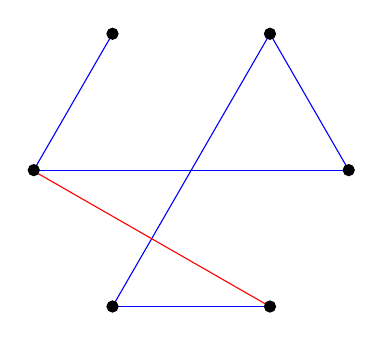
\begin{tikzpicture}
                \draw [blue] (0,0) -- (2,0);
                \draw [blue] (3,1.7321) -- (2,3.4641);
                \draw [blue] (3,1.7321) -- (-1,1.7321);
                \draw [blue] (0,3.4641) -- (-1,1.7321);
                \draw [blue] (0,0) -- (2,3.4641);
        
                \draw [red] (-1,1.72,0) -- (2,0);
        
                \filldraw (0,0) circle (2pt);
                \filldraw (2,0) circle (2pt);
                \filldraw (3,1.7321) circle (2pt);
                \filldraw (2,3.4641) circle (2pt);
                \filldraw (0,3.4641) circle (2pt);
                \filldraw (-1,1.7321) circle (2pt);
            \end{tikzpicture}
        
        \end{center}       
    \end{figure}
    
\end{frame} 

\begin{frame}
    \frametitle{A motivational example}

    \begin{figure}[h]
        \begin{center}
            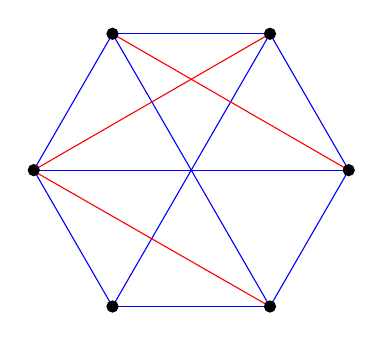
\begin{tikzpicture}
                \draw [blue] (0,0) -- (2,0);
                \draw [blue] (2,0) -- (3,1.7321);
                \draw [blue] (3,1.7321) -- (2,3.4641);
                \draw [blue] (2,3.4641) -- (0,3.4641);
                \draw [blue] (0,3.4641) -- (-1,1.7321);
                \draw [blue] (-1,1.7321) -- (0,0);
                \draw [blue] (0,0) -- (2,3.4641);
                \draw [blue] (3,1.7321) -- (-1,1.7321);
                \draw [blue] (2,0) -- (0,3.4641);
        
                \draw [red] (3,1.7321) -- (0,3.4641);
                \draw [red] (2,3.4641) -- (-1,1.7321);
                \draw [red] (-1,1.72,0) -- (2,0);
        
                \filldraw (0,0) circle (2pt);
                \filldraw (2,0) circle (2pt);
                \filldraw (3,1.7321) circle (2pt);
                \filldraw (2,3.4641) circle (2pt);
                \filldraw (0,3.4641) circle (2pt);
                \filldraw (-1,1.7321) circle (2pt);
            \end{tikzpicture}
        
        \end{center}       
    \end{figure}
    
\end{frame} 

\begin{frame}
    \frametitle{A motivational example}

    \begin{figure}[h]
        \begin{center}
            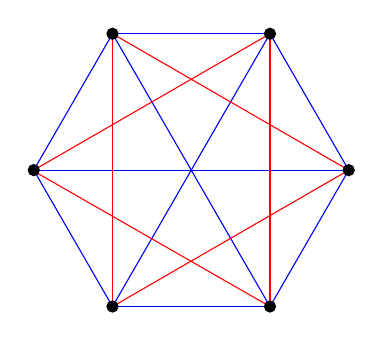
\begin{tikzpicture}
                \draw [blue] (0,0) -- (2,0);
                \draw [blue] (2,0) -- (3,1.7321);
                \draw [blue] (3,1.7321) -- (2,3.4641);
                \draw [blue] (2,3.4641) -- (0,3.4641);
                \draw [blue] (0,3.4641) -- (-1,1.7321);
                \draw [blue] (-1,1.7321) -- (0,0);
                \draw [blue] (0,0) -- (2,3.4641);
                \draw [blue] (3,1.7321) -- (-1,1.7321);
                \draw [blue] (2,0) -- (0,3.4641);
        
                \draw [red] (0,0) -- (3,1.7321);
                \draw [red] (3,1.7321) -- (0,3.4641);
                \draw [red] (0,3.4641) -- (0,0);
                \draw [red] (2,0) -- (2,3.4641);
                \draw [red] (2,3.4641) -- (-1,1.7321);
                \draw [red] (-1,1.72,0) -- (2,0);
        
                \filldraw (0,0) circle (2pt);
                \filldraw (2,0) circle (2pt);
                \filldraw (3,1.7321) circle (2pt);
                \filldraw (2,3.4641) circle (2pt);
                \filldraw (0,3.4641) circle (2pt);
                \filldraw (-1,1.7321) circle (2pt);
            \end{tikzpicture}
        
        \end{center}  
        \caption{2 red triangles within a graph of 6 vertices}     
    \end{figure}
    
\end{frame} 

Notice that if adding a seventh vertex does not affect the existence of the monochromatic 
triangles. In fact adding any number of vertices to graph doesn't affect this. 
However, if we take a vertex away from the graph and consider the edge colouring 
shown here, we can't find any red or blue triangles.

\begin{frame}
    \frametitle{A pathological example}

    \begin{figure}[h]
        \begin{center}
            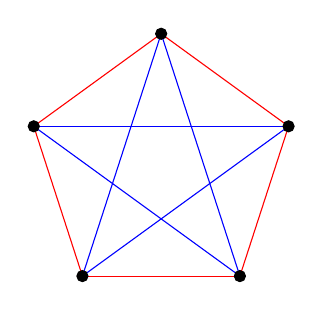
\begin{tikzpicture}
                \draw [red] (0,0) -- (2,0);
                \draw [red] (2,0) -- (2.618,1.9022);
                \draw [red] (2.618,1.9022) -- (1,3.0776);
                \draw [red] (1,3.0776) -- (-0.618,1.9022);
                \draw [red] (-0.618,1.9022) -- (0,0);

                \draw [blue] (0,0) -- (2.618,1.9022);
                \draw [blue] (0,0) -- (1,3.0776);
                \draw [blue] (2,0) -- (1,3.0776);
                \draw [blue] (2,0) -- (-0.618,1.9022);
                \draw [blue] (2.618,1.9022) -- (-0.618,1.9022);
        
                \filldraw (0,0) circle (2pt);
                \filldraw (2,0) circle (2pt);
                \filldraw (2.618,1.9022) circle (2pt);
                \filldraw (1,3.0776) circle (2pt);
                \filldraw (-0.618,1.9022) circle (2pt);
            \end{tikzpicture}
        
        \end{center}
        
        \caption{A particular 2-colouring of $K_5$}
    \end{figure}

\end{frame}

So we have found that 6 is minimum 
number of vertices needed in to ensure the existence of monochromatic triangles. This motivates 
the definition of Ramsey numbers.

First some definitions:

\begin{frame}
    \frametitle{Definitions}

    By \textit{$r$-colouring} of a graph $G=(V,E)$, we mean a partition of the edges $E$ 
    induced by the map 
    $$\chi: E \to \{1,2,\ldots,r\},text{     for } r\in\Z^+.$$
    We say a subset of edges $E'\subset E$ is monochromatic if the restriction 
    $\chi|_{E'}$ is the constant map.

    We say a graph is \textit{complete} if every two vertices are joined by an edge. 
    We denote the complete graph of order $n$ $K_n$, where the order of a graph is 
    the number of vertices. 
\end{frame}

\begin{frame}
    \frametitle{Ramsey numbers}

    \begin{definition}[Ramsey number]

        For $s,t\in\Z^+$, we define the \textit{Ramsey number} of $s$ and $t$, $R(s,t)$, 
        to be the least positive integer such that any 2-colouring of $K_n$ contains
        as a subgraph a monochromatic $K_s$ or a monochromatic $K_t$, whenever 
        $n\geq R(s,t)$.
    
    \end{definition}
\end{frame}

\begin{frame}
    \frametitle{Ramsey's theorem}

    \begin{prop}
    $R(s,t)$ is a well-defined function for all $s,t\in\Z^+$, and
    
    \end{prop}

\end{frame}

\begin{frame}
    \frametitle{Generalisation}
    In fact, we can colour the edges of a graph with any finite number of colours, 
    and Ramsey's theorem still holds. For $s_1,\ldots,s_r\in\Z^+$, we define the $R(s_1,\ldots,s_r)$, 
    to be the least positive integer such that any 2-colouring of $K_n$ contains
    as a subgraph a monochromatic $K_s$ or a monochromatic $K_t$, whenever 
    $n\geq R(s,t)$.

\end{frame}